\documentclass[12pt, twoside]{article}
\usepackage[utf8]{inputenc}
\usepackage[english,russian]{babel}

\usepackage{amsthm}
\usepackage{a4wide}
\usepackage{graphicx}
\usepackage{caption}
\usepackage{amssymb}
\usepackage{amsmath}
\usepackage{mathrsfs}
\usepackage{euscript}
\usepackage{graphicx}
\usepackage{subfig}
\usepackage{caption}
\usepackage{color}
\usepackage{bm}
\usepackage{tabularx}
\usepackage{adjustbox}


\usepackage[toc,page]{appendix}

\usepackage{comment}
\usepackage{rotating}

\DeclareMathOperator*{\argmax}{arg\,max}
\DeclareMathOperator*{\argmin}{arg\,min}

\newtheorem{theorem}{Теорема}
\newtheorem{lemma}[theorem]{Лемма}
\newtheorem{definition}{Определение}[section]

\numberwithin{equation}{section}

\newcommand*{\No}{No.}
\begin{document}

\title{\bf Анализ выбора априорного распределения для смеси экспертов \thanks{Работа выполнена при поддержке РФФИ и правительства РФ.}}
\date{}
\author{}
\maketitle

\begin{center}
\bf
А.\,В.~Грабовой\footnote{Московский физико-технический институт, grabovoy.av@phystech.edu}, В.\,В.~Стрижов\footnote{Московский физико-технический институт, strijov@ccas.ru}

\end{center}

{\centering\begin{quote}
\textbf{Аннотация:} 
Данная работа посвящен анализу свойств смеси экспертов в зависимости от выбора априорного распределения. Анализируется случай, когда выбрано информативное и неинформативное априорное распределения весов параметров каждого эксперта. В качестве экспертов рассматриваются линейные модели, а в качестве гипермодели рассматривается нейросеть с функцией softmax на последнем слое. В качестве базовой задачи рассматривается задача поиска окружностей на изображении. Предполагается, что каждой окружности на изображении соответсвует свой эксперт. В качестве данных рассматриваются синтетически сгенерированные окружности с разным уровнем шума. Сравнивается устойчивость к шуму мультимомделей с задаными априорными распределениями на вектора параметров локальных моделей и без задания априорного распределения.

\smallskip
\textbf{Ключевые слова}: смесь экспертов; байесовский выбор модели; априорное распределение.

\smallskip
\textbf{DOI}: 00.00000/00000000000000
\end{quote}
}

\section{Введение}
В данной работе рассматривается задача смеси экспертов. Смесь экспертов --- это мультимодель, которая линейно взвешивает результаты других моделей для конечного результата, причем коэффициенты взвешивания зависят от объекта для которого производится предсказаниие.

Мультимодели показывают отличные результаты во многих задачах. Классическими методами являются беггинг и градиентный бустинг~\cite{Tianqi2016}, случайный лес~\cite{Ishwaran2012}. Подход к мультимоделированию~\cite{Yuksel2012} предполагает, что вклад каждой модели в ответ должен зависеть от конкретного объекта. Смесь экспертов базируется на понятии шлюзовой функции, которая определяет значимость предсказания каждого эксперта --- отдельной модели.

Для поиска оптимальных параметров рассматривается вероятностная постановка задачи. В качестве функционала качества рассматривается логарифм правдоподобие модели. Для оптимизации данного функционала рассматривается EM-алгоритм.

Несмотря на значимые успехи мультимоделей, они имеют ряд недостатков. Данные недостатки связаны с тем, что сходимость локальных моделей сильно зависит от начальной инициализации векторов параметров. Для улучшения сходимости предлагается использовать априорные знание о данных.

\begin{figure}[h!t]\center
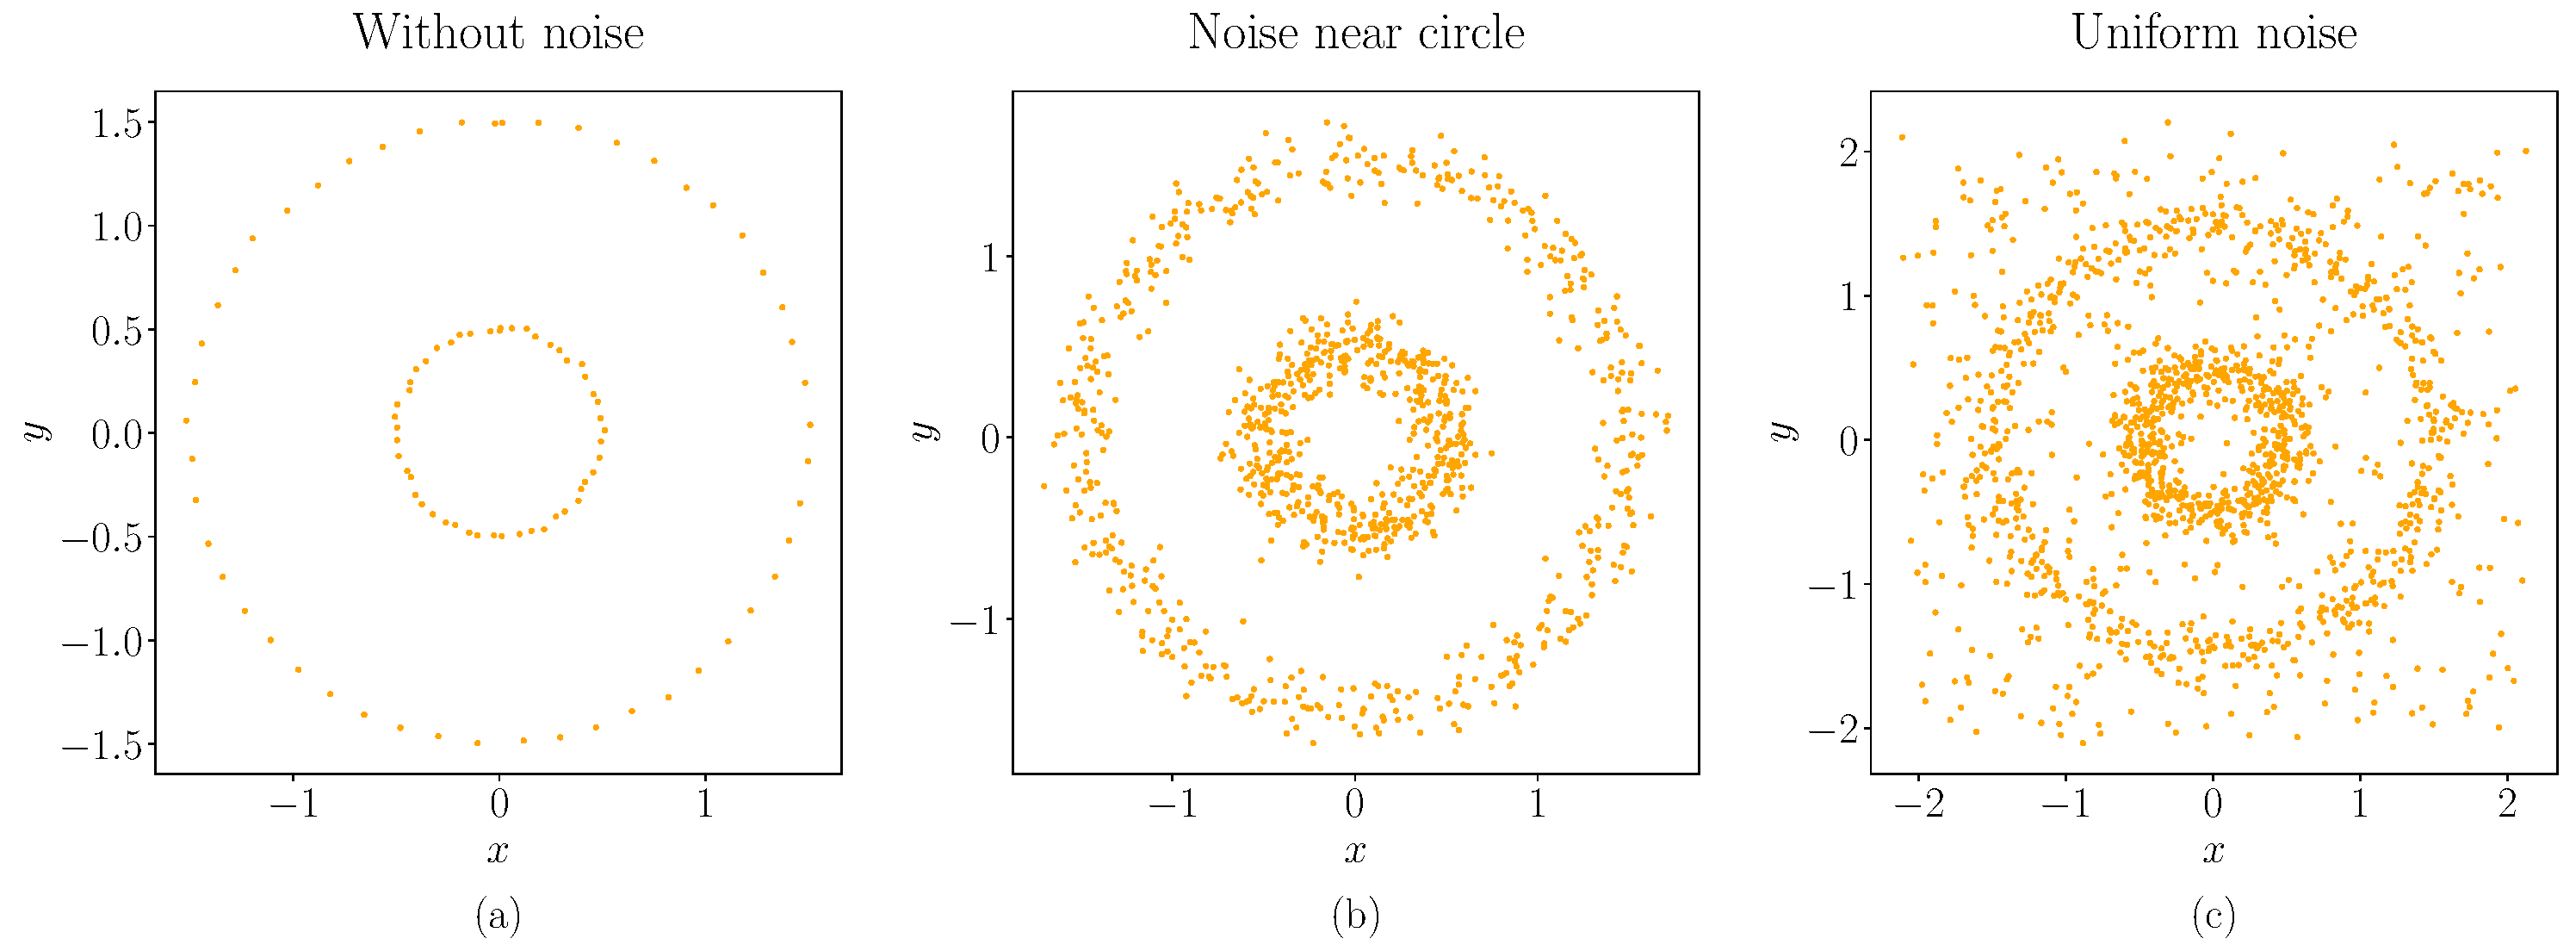
\includegraphics[width=1\textwidth]{results/statment}
\caption{Пример изображений с окружностями с разным уровнем шума: a) окружности без шума; b) окружности с зашумленным радиусом; c) окружности с зашумленным радиусом, а также с равномерным шумом по всему изображению}
\label{example:1}
\end{figure}

Данная работа исследует, влияние выбора априорного распределения параметров моделей на сходимость мультимодели. Решается задача поиска окружностей на бинаризованном изображении. Предполагается, что радиусы окружностей различаются значимо. Пример изображений показан на рис.~\ref{example:1}. Предлагается рассмотреть как ведет себя модель с априорными знанием и без них в случае изображений с разным уровнем шума. В данной работе в качестве отдельных экспертов рассматриваются линейные модели --- каждая модель отвечает своей окружности. В качестве шлюзовой функции рассматривается двухслойная нейронная сеть.

\section{Работы по теме}
Большое количество работ посвящены выбору шлюзовой функции: softmax--регрессия, процесс Дирихле~\cite{Edward2002}, нейронная сеть~\cite{Shazeer2017} с softmax на последнем слое.

Ряд работ посвящены выбору моделей в качестве отдельных экспертов. В работах~\cite{Jordan1994, Jordan1991} в качестве модели эксперта рассматривается линейная модель --- гаусиана. Работы~\cite{Lima2007, Cao2003} рассматриваю модель SVM в качестве модели эксперта.

В работа~\cite{Yuksel2012} представлен обзор методов и моделей в задачах смеси экспертов. В данной работе представлен обзор выше перечисленных шлюзовых функций. Также в данной работе проведен анализ разных моделей, которые могут выступать в качестве локальной модели.


\section{Постановка задачи нахождения параметров окружностей}
Задано бинарное изображение:
\begin{equation}
\label{eq:st:cr:1}
\begin{aligned}
\textbf{M} \in \{0,1\}^{m_1 \times m_2},
\end{aligned}
\end{equation}
где $0$ отвечает белой точке --- фону, $1$ --- черная точке изображения.

По изображению $\textbf{M}$ строится выборка $\textbf{C}$, элементами которой являются координаты~$x_i, y_i$ черных точек на картинке:
\begin{equation}
\label{eq:st:cr:2}
\begin{aligned}
\textbf{C} \in  \mathbb{R}^{N \times 2},
\end{aligned}
\end{equation}
где $N$ --- количество черных точек на изображении $\textbf{M}$.

Обозначим $x_0, y_0$ --- центр окружности, которую требуется найти на бинарном изображении $\textbf{M}$, а $r$ ее радиус. Тогда элементы выборки $\textbf{C}$ должны удовлетворять уравнению окружности:
\begin{equation}
\label{eq:st:cr:3}
\begin{aligned}
\left(x_i - x_0\right)^{2}+\left(y_i-y_0\right)^2 = r^2.
\end{aligned}
\end{equation}
Раскрыв скобки получим следующие уравнение:
\begin{equation}
\label{eq:st:cr:4}
\begin{aligned}
(2x_0)\cdot x_i + (2y_0)\cdot y_i+(r^2-x_0^2-y_0^2)\cdot1 = x_{i}^2 + y_{i}^2.
\end{aligned}
\end{equation}
Получаем задачу линейной регрессии для нахождения параметров окружности:
\begin{equation}
\label{eq:st:cr:5}
\begin{aligned}
\textbf{X}\textbf{w} \approx \textbf{Y},  \quad \textbf{X} = \textbf{C}\times \textbf{1}, \quad \textbf{Y} = \{x^2+y^2|~\forall x,y \in \textbf{C}\},
\end{aligned}
\end{equation}
где найденые оптимальные параметры линейной регрессии $\textbf{w} = \{w_1, w_2, w_3\}$ восстанавливают параметры окружности:
\begin{equation}
\label{eq:st:cr:6}
\begin{aligned}
x_0 = \frac{w_1}{2}, \quad y_0 = \frac{w_2}{2}, \quad r = \sqrt[]{w_3+x_{0}^{2}+y_{0}^{2}}.
\end{aligned}
\end{equation}

Данное решение позволяет искать параметры единственной окружности на рисунке. В случае, когда на картинке несколько окружностей предлагается использовать мультимодель, где в качестве каждой модели рассматривается единственная линейная модель, которая отвечает одной окружности на рисунке. В качестве мультимодели рассматривается смесь экспертов.

\section{Постановка задачи построения смеси экспертов}

Задана выборка
\begin{equation}
\label{eq:st:1}
\begin{aligned}
\textbf{X} \in \mathbb{R}^{N \times n},
\end{aligned}
\end{equation}
где~$N$~---~число объектов в выборке, а~$n$~---~размерность признакового пространства.

\begin{definition}
Смесь экспертов~---~мультимодель, определяющая правдоподобие веса $\pi_k$ каждой модели $\textbf{f}_k$ на признаковом описании объекта $\textbf{x}$.

\begin{equation}
\label{eq:st:2}
\begin{aligned}
\hat{\mathbf{f}} = \sum_{k=1}^{K}\pi_{k}\mathbf{f}_k, \qquad \pi_{k}\left(\textbf{x}, \textbf{V}\right):\mathbb{R}^{2\times n} \to [0, 1], \qquad \sum_{k=1}^{K}\pi_{k}\left(\textbf{x}, \textbf{V}\right) = 1
\end{aligned}
\end{equation}
где~$\hat{\mathbf{f}}$~---~мультимодель, а $\mathbf{f}_k$ является некоторой моделью, $\pi_k$~---~параметрическая модель.
\end{definition}

\begin{figure}[h!t]\center
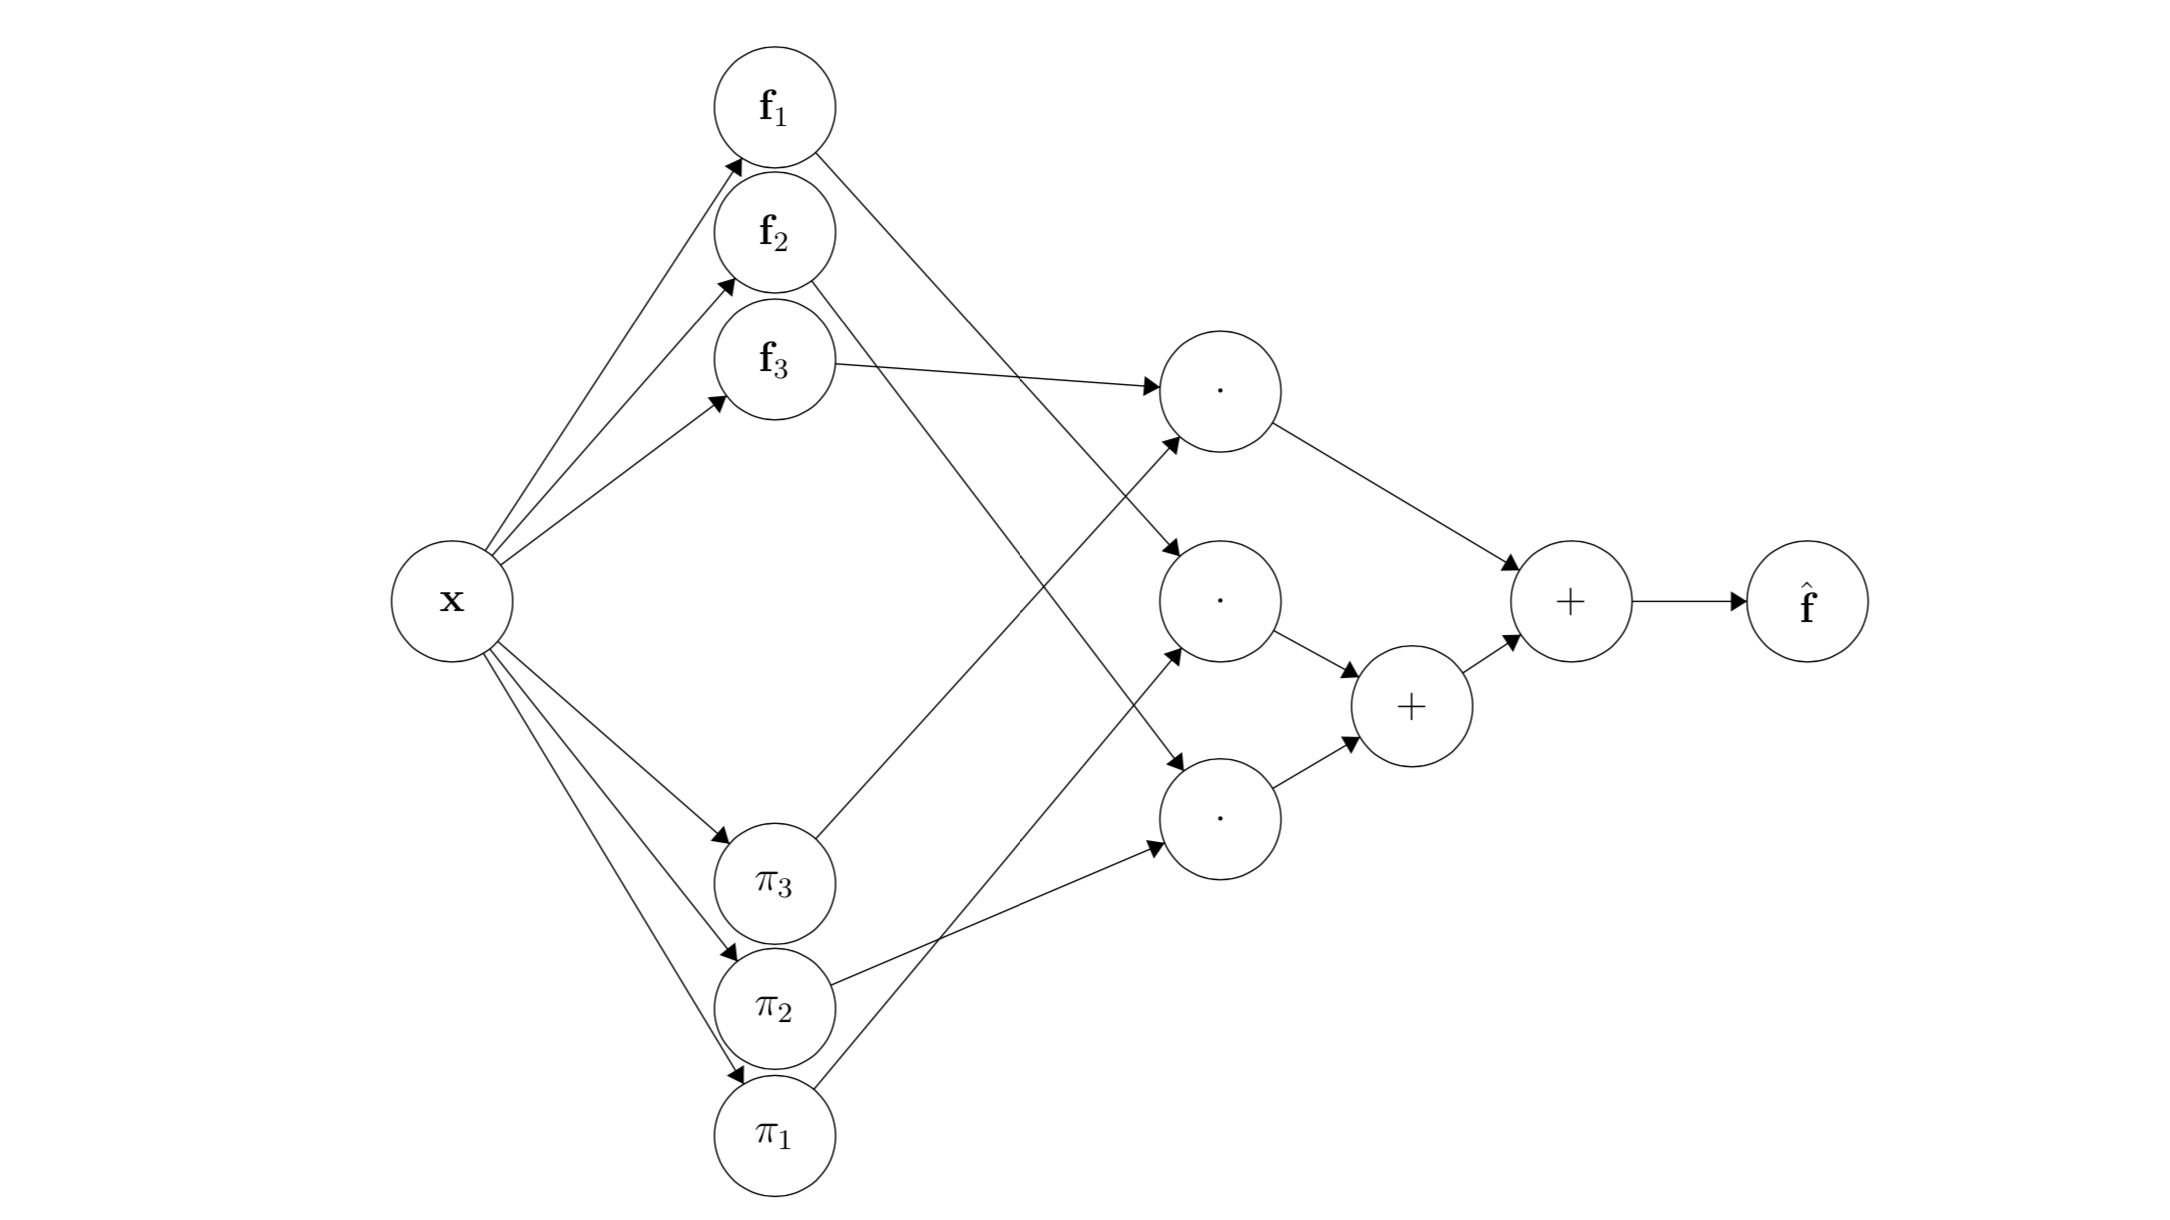
\includegraphics[width=1\textwidth]{results/scheme}
\caption{Схема смеси экспертов, в случае трех локальных моделей: $\textbf{f}_k$~---~локальные модели, $\pi_k$~---~шлюзовая функция, $\hat{\mathbf{f}}$~---~мультимодель. Каждая стрелка обозначает то, что объект от которого исходит стрелка подставляется в ту функция, где стрелка заканчивается.}
\label{scheme:1}
\end{figure}

На рис.~\ref{scheme:1} показан пример мультимодели, которая изображена при помощи графовой нотации. В данном примере число локальных моделей $\textbf{f}_k$ равняется трем.

\subsection{Общий случай}
В качестве моделей рассматриваются произвольные параметрические функции. В качестве шлюзовой функции, также рассматривается произвольная параметрическая функция. Подразумевается, что существует производная выхода модели по вектору ее параметров. Поиск параметров мультимодели производится при помощи максимизации правдоподобия модели, которое рассматривается как функция качества модели. Оптимизация параметров проводится при помощи ЕМ-алгоритма.

Правдоподобие модели:
\begin{equation}
\label{eq:st:3}
\begin{aligned}
p\left(\textbf{y}, \textbf{W}, \textbf{Z}|\textbf{X}, \textbf{V}, \textbf{W}^{0}, \textbf{A}\right) &= \prod_{i=1}^{N}\prod_{k=1}^{K}\left[\pi_{k}\left(\textbf{x}_i,\textbf{V}\right)p_k\left(y_i|\textbf{w}_{k}, \textbf{x}_i\right)\right]^{z_{ik}}\prod_{k=1}^{K}p^{k}\left(\textbf{w}_{k}|\textbf{w}^{0}_{k}, \textbf{A}_{k}\right)
\end{aligned}
\end{equation}

Рассмотрим логарифм правдоподобия модели, чтобы функция качества модели была линейной функцией по объектам выборки:
\begin{equation}
\label{eq:st:4}
\begin{aligned}
\log p\left(\textbf{y}, \textbf{W}, \textbf{Z}|\textbf{X}, \textbf{V}, \textbf{W}^{0}, \textbf{A}\right) &= \sum_{i=1}^{N}\sum_{k=1}^{K}z_{ik}\left[\log\pi_k\left(\textbf{x}_i, \textbf{V}\right) + \log p_k\left(y_i|\textbf{w}_{k}, \textbf{x}_{i}\right)\right] +\\
&+ \sum_{k=1}^{K}\log p^{k}\left(\textbf{w}_{k}|\textbf{w}^{0}_{k}, \textbf{A}_{k}\right)
\end{aligned}
\end{equation}

Используя EM-алгоритм получим формулы для поиска оптимальных параметров при помощи итерационного процесса. 
\paragraph{E-step}~

Найдем $q\left(\textbf{Z}\right)$:
\begin{equation}
\label{eq:st:5}
\begin{aligned}
\log q\left(\textbf{Z}\right) &= \mathsf{E}_{q/\textbf{Z}}\log p\left(\textbf{y}, \textbf{W}, \textbf{Z}|\textbf{X}, \textbf{V}, \textbf{W}^{0}, \textbf{A}\right) \\
p\left(z_{ik} = 1\right) &= \frac{\exp\left(\log\pi_{k}\left(\textbf{x}_{i}, \textbf{V}\right) + \mathsf{E}\log p_{k}\left(y_i|\textbf{w}_k, \textbf{A}_k\right)\right)}{\sum_{k'=1}^{K}\exp\left(\log\pi_{k'}\left(\textbf{x}_{i}, \textbf{V}\right) + \mathsf{E}\log p_{k'}\left(y_i|\textbf{w}_k', \textbf{A}_k'\right)\right)}
\end{aligned}
\end{equation}

Найдем $q\left(\textbf{W}\right)$:
\begin{equation}
\label{eq:st:6}
\begin{aligned}
\log q\left(\textbf{W}\right) &= \mathsf{E}_{q/\textbf{W}}\log p\left(\textbf{y}, \textbf{W}, \textbf{Z}|\textbf{X}, \textbf{V}, \textbf{W}^{0}, \textbf{A}\right) \\
&= \sum_{i=1}^{N}\sum_{k=1}^{K}\mathsf{E}z_{ik}\left[\log\pi_{k}\left(\textbf{x}_{i, \textbf{V}}\right) + \log p_{k}\left(y_{i}\left(y_{i}|\textbf{w}_{k}, \textbf{x}_i\right)\right)\right] + \\
&+ \sum_{k=1}^{K}\log p^{k}\left(\textbf{w}_{k}|\textbf{w}^{0}_{k}, \textbf{A}_{k}\right)
\end{aligned}
\end{equation}

\paragraph{M-step}~
\begin{equation}
\label{eq:st:7}
\begin{aligned}
\mathsf{E}_{q} p\left(\textbf{y}, \textbf{W}, \textbf{Z}|\textbf{X}, \textbf{V}, \textbf{W}^{0}, \textbf{A}\right) &= \mathcal{F}\left(\textbf{V}, \textbf{W}^{0}, \textbf{A}\right) \\
\mathcal{F}\left(\textbf{V}, \textbf{W}^{0}, \textbf{A}\right) &= \sum_{i=1}^{N}\sum_{k=1}^{K}\mathsf{E}z_{ik}\left[\log\pi_k\left(\textbf{x}_i, \textbf{V}\right) + \mathsf{E}\log p_{k}\left(y_i|\textbf{w}_{k}, \textbf{x}_{i}\right)\right] \\
&+ \sum_{k=1}^{K}\mathsf{E}\log p_{k}\left(\textbf{w}_{k}|\textbf{w}^{0}_{k}, \textbf{A}_{k}\right)
\end{aligned}
\end{equation}

Найдем $\textbf{A}$ из условия
\begin{equation}
\label{eq:st:8}
\begin{aligned}
\frac{\partial \mathcal{F}\left(\textbf{V}, \textbf{W}^{0}, \textbf{A}\right)}{\partial \textbf{A}^{-1}} = 0.
\end{aligned}
\end{equation}

Найдем $\textbf{V}$ из условия
\begin{equation}
\label{eq:st:9}
\begin{aligned}
\frac{\partial \mathcal{F}\left(\textbf{V}, \textbf{W}^{0}, \textbf{A}\right)}{\partial \textbf{V}} = 0.
\end{aligned}
\end{equation}

Найдем $\textbf{W}^{0}$ из условия
\begin{equation}
\label{eq:st:10}
\begin{aligned}
\frac{\partial \mathcal{F}\left(\textbf{V}, \textbf{W}^{0}, \textbf{A}\right)}{\partial \textbf{W}^{0}} = 0.
\end{aligned}
\end{equation}

\subsection{Случай линейной регресионной модели}
В данной задаче рассматривается случай линейных локальных моделей. В этом случае неизвестные функции из общего вида превращаются в явный вид:
\begin{enumerate}
	\item $p_{k}\left(y_{i}|\textbf{w}_{k}, \textbf{x}_{i}\right) = \text{N}\left(y_{i}|\textbf{w}_{k}^{\mathsf{T}}\textbf{x}_{i}, \beta^{-1}\right)$
	\item $p^{k}\left(\textbf{w}_{k}|\textbf{w}^{0}_{k}, \textbf{A}_{k}\right) = \text{N}\left(\textbf{w}_{k}|\textbf{w}^{0}_{k}, \textbf{A}_{k}\right)$
	\item $\bm{\pi}\left(\textbf{x}_{i}, \textbf{V}\right) = \text{softmax}\left(\textbf{F}\left(\textbf{x}_{i}, \textbf{V}\right)\right),$ где $F : \mathbb{R}^{n}\times\mathbb{R}^{V}\to \mathbb{R}^{K}$ --- нейросеть, V --- число параметров нейросети. 
\end{enumerate}


С учетом наших предположений логарифм правдоподобия переписывается в следующем виде:
\begin{equation}
\label{eq:st:lin:2}
\begin{aligned}
\log p\left(\textbf{y}, \textbf{W}, \textbf{Z}|\textbf{X}, \textbf{V}, \textbf{W}^{0}, \textbf{A}\right) &= \sum_{i=1}^{N}\sum_{k=1}^{K}z_{ik}\left[\log\pi_k\left(\textbf{x}_i, \textbf{V}\right) - \frac{\beta}{2}\left(y_{i} - \textbf{w}_{k}^{\mathsf{T}}\textbf{x}_{i}\right)^{2} + \frac{1}{2}\log\frac{\beta}{2\pi}\right] +\\
&+ \sum_{k=1}^{K}\left[-\frac{1}{2}\left(\textbf{w}_{k} - \textbf{w}_{k}^{0}\right)^{\mathsf{T}}\textbf{A}_{k}^{-1}\left(\textbf{w}_{k} - \textbf{w}_{k}^{0}\right) + \frac{1}{2}\log\det\textbf{A}^{-1}_{k} - \frac{n}{2}\log2\pi\right]
\end{aligned}
\end{equation}

Воспользуемся ЕМ-алгоритмом для решения оптимизационной задачи. В случае ограничений, которые предложены в данном разделе получим явный вид итерационных формул.

\paragraph{E-step}~

Найдем $q\left(\textbf{Z}\right)$:
\begin{equation}
\label{eq:st:lin:3}
\begin{aligned}
\log q\left(\textbf{Z}\right) &= \mathsf{E}_{q/\textbf{Z}}\log p\left(\textbf{y}, \textbf{W}, \textbf{Z}|\textbf{X}, \textbf{V}, \textbf{W}^{0}, \textbf{A}\right)  \propto\\
&\propto \sum_{i+1}^{N}\sum_{k=1}^{K}z_{ik}\left[\log\pi_{k}\left(\textbf{x}_{i}, \textbf{V}\right) - \frac{\beta}{2}\left(y_{i}^{2} -\textbf{x}_{i}^{\mathsf{T}}\mathsf{E}\textbf{w}_{k} + \textbf{x}_{i}^{\mathsf{T}}\mathsf{E}\textbf{w}_{k}\textbf{w}_{k}^{\mathsf{T}}\textbf{x}_{i}\right) + \frac{1}{2}\log\frac{\beta}{2\pi}\right]\\
p\left(z_{ik} = 1\right) &= \frac{\exp\left(\log\pi_{k}\left(\textbf{x}_{i}, \textbf{V}\right) - \frac{\beta}{2}\left(\textbf{x}_{i}^{\mathsf{T}}\mathsf{E}\textbf{w}_{k}\textbf{w}_{k}^{\mathsf{T}}\textbf{x}_{i} - \textbf{x}_{i}^{\mathsf{T}}\mathsf{T}\textbf{w}_{k}\right)\right)}{\sum_{k'=1}^{K}\exp\left(\log\pi_{k'}\left(\textbf{x}_{i}, \textbf{V}\right) - \frac{\beta}{2}\left(\textbf{x}_{i}^{\mathsf{T}}\mathsf{E}\textbf{w}_{k'}\textbf{w}_{k'}^{\mathsf{T}}\textbf{x}_{i} - \textbf{x}_{i}^{\mathsf{T}}\mathsf{T}\textbf{w}_{k'}\right) \right)}
\end{aligned}
\end{equation}

Найдем $q\left(\textbf{W}\right)$:
\begin{equation}
\label{eq:st:lin:4}
\begin{aligned}
\log q\left(\textbf{W}\right) &= \mathsf{E}_{q/\textbf{W}}\log p\left(\textbf{y}, \textbf{W}, \textbf{Z}|\textbf{X}, \textbf{V}, \textbf{W}^{0}, \textbf{A}\right) \\
&= \sum_{i=1}^{N}\sum_{k=1}^{K}\mathsf{E}z_{ik}\left[\log\pi_{k}\left(\textbf{x}_{i, \textbf{V}}\right) - \frac{\beta}{2}\left(y_{i} - \textbf{w}_{k}^{\mathsf{T}}\textbf{x}_{i}\right)^{2} + \frac{1}{2}\log\frac{\beta}{2\pi}\right] + \\
&+ \sum_{k=1}^{K}\left[-\frac{1}{2}\left(\textbf{w}_{k} - \textbf{w}_{k}^{0}\right)^{\mathsf{T}}\textbf{A}_{k}^{-1}\left(\textbf{w}_{k} - \textbf{w}_{k}^{0}\right) + \frac{1}{2}\log\det\textbf{A}^{-1}_{k} - \frac{n}{2}\log2\pi\right] \\
&= \sum_{k=1}^{K}\left[\textbf{w}_{k}^{\mathsf{T}}\left(\textbf{A}_{k}^{-1}\textbf{w}_{k}^{0}+\beta\sum_{i=1}^{N}\textbf{x}_{i}y_{i}\mathsf{E}z_{ik}\right)-\frac{1}{2}\textbf{w}_{k}^{\mathsf{T}}\left(\textbf{A}_{k}^{-1}+\beta\sum_{i=1}^{N}\textbf{x}_{i}\textbf{x}_{i}^{\mathsf{T}}\right)\textbf{w}_{k}\right]
\end{aligned}
\end{equation}

Получаем распределение параметров:
\begin{equation}
\label{eq:st:lin:5}
\begin{aligned}
q\left(\textbf{w}_{k}\right) = \text{N}\left(\textbf{w}_{k}| \textbf{m}_{k}, \textbf{B}_k\right), 
\end{aligned}
\end{equation}
где введены обозначения
\begin{equation}
\label{eq:st:lin:6}
\begin{aligned}
\textbf{m}_{k} = \textbf{B}_{k}\left(\textbf{A}_{k}^{-1}\textbf{w}_{k}^{0}+\beta\sum_{i=1}^{N}\textbf{x}_{i}y_{i}\mathsf{E}z_{ik}\right) \qquad \textbf{B}_{k} = \left(\textbf{A}_{k}^{-1}+\beta\sum_{i=1}^{N}\textbf{x}_{i}\textbf{x}_{i}^{\mathsf{T}}\right)^{-1}
\end{aligned}
\end{equation}

\paragraph{M-step}~
\begin{equation}
\label{eq:st:lin:6}
\begin{aligned}
\mathsf{E}_{q} \log p\left(\textbf{y}, \textbf{W}, \textbf{Z}|\textbf{X}, \textbf{V}, \textbf{W}^{0}, \textbf{A}\right) &= \mathcal{F}\left(\textbf{V}, \textbf{W}^{0}, \textbf{A}\right) \\
\mathcal{F}\left(\textbf{V}, \textbf{W}^{0}, \textbf{A}\right) &= \sum_{i=1}^{N}\sum_{k=1}^{K}\mathsf{E}z_{ik}\left[\log\pi_k\left(\textbf{x}_i, \textbf{V}\right) - \frac{\beta}{2}\mathsf{E}\left(y_{i} - \textbf{w}_{k}^{\mathsf{T}}\textbf{x}_{i}\right)^{2} + \frac{1}{2}\log\frac{\beta}{2\pi}\right] +\\
&+ \sum_{k=1}^{K}\left[-\frac{1}{2}\mathsf{E}\left(\textbf{w}_{k} - \textbf{w}_{k}^{0}\right)^{\mathsf{T}}\textbf{A}_{k}^{-1}\left(\textbf{w}_{k} - \textbf{w}_{k}^{0}\right) + \frac{1}{2}\log\det\textbf{A}^{-1}_{k} - \frac{n}{2}\log2\pi\right]
\end{aligned}
\end{equation}

Найдем $\textbf{A}$ из условия:
\begin{equation}
\label{eq:st:lin:7}
\begin{aligned}
\frac{\partial \mathcal{F}\left(\textbf{V}, \textbf{W}^{0}, \textbf{A}_{k}\right)}{\partial \textbf{A}^{-1}} =  \frac{1}{2}\textbf{A}_{k} - \frac{1}{2}\mathsf{E}\left(\textbf{w}_{k} - \textbf{w}_{k}^{0}\right)\left(\textbf{w}_{k} - \textbf{w}_{k}^{0}\right)^{T} = 0 
\end{aligned}
\end{equation}

Получаем $\textbf{A}$:
\begin{equation}
\label{eq:st:lin:8}
\begin{aligned}
\textbf{A}_{k} = \mathsf{E}\textbf{w}_{k}\textbf{w}_{k}^{\mathsf{T}} - 2\textbf{w}_{k}^{0}\mathsf{E}\textbf{w}_{k}^{\mathsf{T}} + \textbf{w}_{k}^{0}\textbf{w}_{k}^{0\mathsf{T}} 
\end{aligned}
\end{equation}

Найдем $\textbf{V}$:

Аналитически решение не ищется, поэтому воспользуемся градиентным спуском для максимизации правдоподобия модели:
\begin{equation}
\label{eq:st:lin:9}
\begin{aligned}
\textbf{V}^{j+1} &= \textbf{V}^{j} + \alpha\frac{\partial \mathcal{F}\left(\textbf{W}, \textbf{V}^{j}, \beta\right)}{\partial \textbf{V}} 
\end{aligned}
\end{equation}

Найдем $\textbf{W}^{0}$ из условия:
\begin{equation}
\label{eq:st:lin:10}
\begin{aligned}
\frac{\partial \mathcal{F}\left(\textbf{V}, \textbf{W}^{0}, \textbf{A}\right)}{\partial \textbf{w}_{k}^{0}} = -2\textbf{A}_{k}^{-1}\mathsf{E}\textbf{w}_{k} + 2\textbf{A}_{k}^{-1}\textbf{w}_{k}^{0}=0
\end{aligned}
\end{equation}

Получаем $\textbf{W}^{0}$:
\begin{equation}
\label{eq:st:lin:11}
\begin{aligned}
\textbf{w}_{k}^{0} = \mathsf{E}\textbf{w}_{k}
\end{aligned}
\end{equation}

\section{Вычислительный эксперимент}
Для сравнения мультимодели смеси экспертов с заданием априорного распределения на вектора параметров локальных моделей и мультимодели без задания априорного распределения на вектора параметров локальных моделей был проведен вычислительный эксперимент на синтетической выборке.

\begin{figure}[h!t]\center
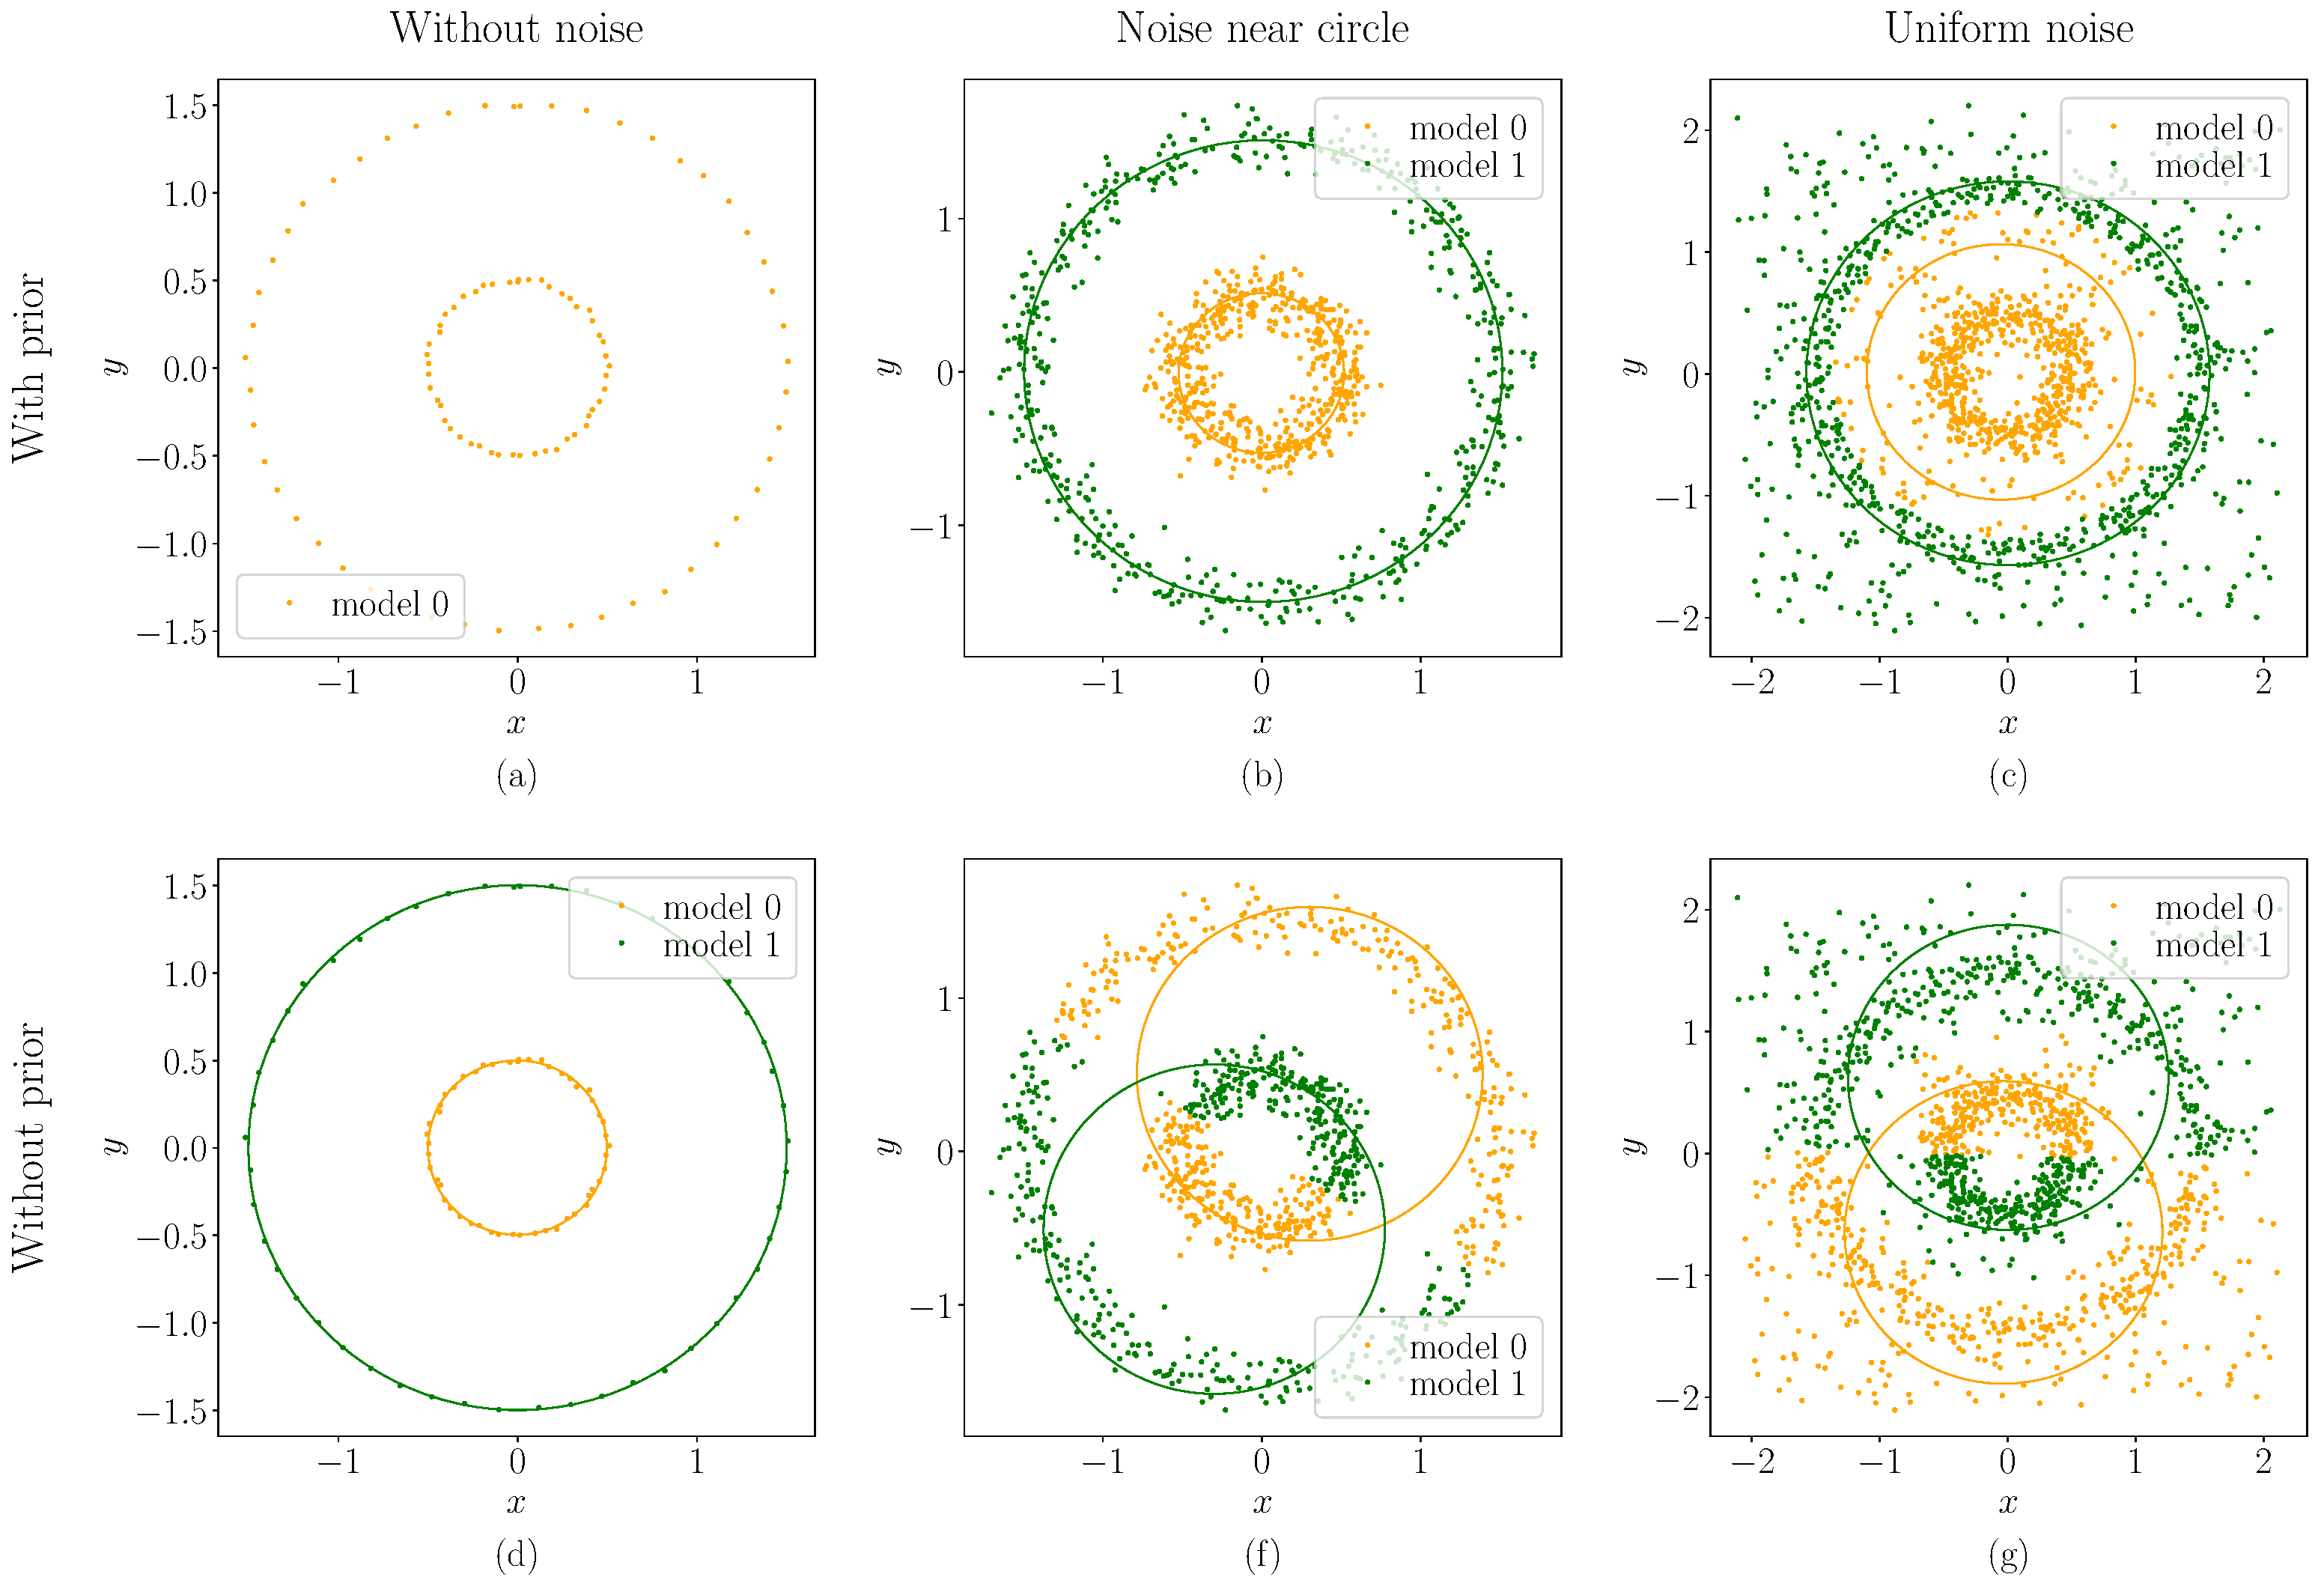
\includegraphics[width=1\textwidth]{results/experiment_synthetic}
\caption{Результат работы мультимодели в зависимости от априорных знаний и в зависимости от уровня шума: a) модель с априорными знаниями, окружности без шума; b) модель с априорными знаниями, окружности с зашумленным радиусом; c) модель с априорными знаниями, окружности с зашумленным радиусом, а также с равномерным шумом по всему изображению; d) модель без априорных знаний, окружности без шума; f) модель без априорных знаний, окружности с зашумленным радиусом; g) модель без априорных знаний, окружности с зашумленным радиусом, а также с равномерным шумом по всему изображению}
\label{experiment:1}
\end{figure}
Вычислительный эксперимент проводится на синтетической выборке, которая получена при помощи генерации двух концентрических окружностей с разным уровнем шума.

Предлагается сравнить две разные постановки задачи смеси экспертов: в случае когда используются априорные знания об картинке и в случае когда априорные знания отсутствуют.

В качестве информативного априорного знания выступает, то, что предполагается что вектора параметров каждой модели имеют следующие распределения:
\begin{equation}
\label{eq:ce:1}
\begin{aligned}
\text{N}\left(\textbf{w}_1|\textbf{w}^{0}_{1}, \textbf{I}\right), \quad \text{N}\left(\textbf{w}_2|\textbf{w}^{0}_{2}, \textbf{I}\right),
\end{aligned}
\end{equation}
где $\textbf{w}^{0}_1 = [0, 0, 0.1],\ \textbf{w}^{0}_2 = [0, 0, 5]$, что указывает, на то, что известно о концентричности окружностей, а также что у них радиусы различны.

\begin{table}[h!t]
\begin{center}
\caption{Результаты работы мультимоделей}
\label{tb:ce:1}
\begin{tabular}{|c|c|c|c|}
\hline
	Мультимодель & Without Noise& Noise near circle& Uniform noise\\
	\hline
	\multicolumn{1}{|l|}{With prior}
	& $99/100$& $97/100$& $95/100$\\
	\hline
	\multicolumn{1}{|l|}{Without prior}
	& $68/100$& $23/100$& $7/100$\\
\hline

\end{tabular}
\end{center}
\end{table}

На рис.~\ref{experiment:1} показан случайный результаты работы мультимоделей с априорными знаниями и без них. На всех картинках обе модели работала $30$ итераций. Так-как сходимость мултимодели очень сильно зависит от начальной инициализации, также был проведен эксперперимент с множественным запуском мултимодели на одной и той же картиинке. Обе модели на каждой картинке запускались по $100$ раз. В таб.~\ref{tb:ce:1} показано сколько мультимоделей правильно отыскали обе окружности на рисунке. Как видно мультимодель с использованием априорных знаний является более стабильной, чем мультимодель, которая не использует никаких априорных знаний.



\section{Заключение}
В данной работе проведено сравнение мультимоделей в случае, когда было задано априорное распределение параметров каждой модели внутри мультимодели и в случае, когда априорного распределения не было. В качестве данных использовались изображения концентрических окружностей с разным уровнем шума. Для поиска окружностей использовались линейные модели. В качестве шлюзовой функции использовалась двухслойная нейросеть.

Как показано в эксперименте в случае, когда введены априорные знания на линейные модели, мультимодель является более устойчивой к шуму. Также в случае задания априорных знаний моделей, мультимодель менее зависит от начальной инициализации, что также позволяет сказать, что модель является более устойчивой к начальной инициализации.

В дальнейшем планируется улучшить мультимодель при помощи задания априорного распределения на шлюзовую функцию. Планируется рассмотреть в качестве моделей не только модели, которые описывают данные, а также модель, которая отвечает за шум в данных. Предполагается, что вероятность шума мала, поэтому важно задать априорного распределение, которое учитывало бы этот факт.

%[2, 59,12,14]

\begin{thebibliography}{99}
\bibitem{Tianqi2016}
	\textit{Chen Tianqi, Guestrin Carlos} XGBoost: A Scalable Tree Boosting System~// KDD ’16 Proceedings of the 22nd ACM SIGKDD International Conference on Knowledge Discovery and Data Mining. 2016.
	
\bibitem{Ishwaran2012}
	\textit{Chen Xi, Ishwaran Hemant} Random Forests for Genomic Data Analysis~// Genomics. 2012. Issues. 99, No 6. pp. 323--329.

\bibitem{Yuksel2012}
	\textit{Yuksel Seniha Esen, Wilson Joseph N., Gader Paul D} Twenty Years of Mixture of Experts~// IEEE Transactions on Neural Networks and Learning Systems. 2012. Issues. 23, No 8. pp. 1177–1193.

\bibitem{Shazeer2017}
	\textit{Noam Shazeer, Azalia Mirhoseini, Krzysztof Maziarz} Outrageously large neural networks: the sparsely-gated mixture-of-experts layer~// ICLR, 2017.

\bibitem{Edward2002}
	\textit{Rasmussen Carl Edward, Ghahramani Zoubin} Infinite Mixtures of Gaussian Process Experts~// Advances in Neural Information Processing Systems 14. 2002. pp. 881–888.
	
\bibitem{Jordan1994}
	\textit{M.~I.~Jordan} Hierarchical mixtures of experts and the EM algorithm~// Neural Comput., vol. 6, no. 2, pp. 181–214, 1994.
	
\bibitem{Lima2007}
	\textit{C.~A.~M.~Lima, A.~L.~V. Coelho, F.~J.~Von~Zuben} Hybridizing mixtures of experts with support vector machines: Investigation into nonlinear dynamic systems identification~// Inf. Sci., vol. 177, no. 10, pp. 2049–2074, 2007.

\bibitem{Cao2003}
	\textit{L.~Cao} Support vector machines experts for time series forecasting~// Neurocomputing, vol. 51, pp. 321–339, Apr. 2003.
	
\bibitem{Jordan1991}
	\textit{M.~I.~Jordan, R.~A.~Jacobs} Hierarchies of adaptive experts~// in Advances in Neural Information Processing Systems. Cambridge, MA: MIT Press, 1991, pp. 985–992.

 \end{thebibliography}

\end{document}

